\documentclass[11pt,a4paper]{article}
\usepackage[T1]{fontenc}
\usepackage[utf8]{inputenc}
\usepackage{lmodern}
\usepackage{textcomp}
\usepackage[left=1.8cm,right=1.8cm,top=2.3cm,bottom=2.2cm,headheight=14pt,headsep=8pt]{geometry}
\usepackage{multicol}
\usepackage{xcolor}
\usepackage{fancyhdr}
\usepackage{graphicx}
\usepackage{array}
\usepackage{amsmath,amssymb}
\usepackage{setspace}
\usepackage{longtable}
\graphicspath{{../}}
\definecolor{ygreen}{RGB}{46,139,87}
\renewcommand{\normalsize}{\fontsize{10.9}{13.4}\selectfont}
\renewcommand{\familydefault}{\rmdefault}
\setlength{\parindent}{0pt}
\setlength{\columnsep}{0.8cm}
\setlength{\columnseprule}{0.4pt}
\setlength{\multicolsep}{3pt plus 1pt minus 1pt}
\renewcommand{\textsubscript}[1]{\ensuremath{_{\text{\fontsize{8}{8}\selectfont #1}}}}
\renewcommand{\textsuperscript}[1]{\ensuremath{^{\text{\fontsize{8}{8}\selectfont #1}}}}
\newcommand{\diqqat}[1]{\par\smallskip\noindent\textbf{Diqqat!} #1\par\medskip}
\newcommand{\javob}{\par\smallskip\noindent\textbf{Javob:} \rule[-2pt]{7.5cm}{0.4pt}\par\smallskip\noindent\textbf{Diqqat!} Javobingizni javoblar varaqasiga ko`chirib yozing.\par\medskip}
\pagestyle{fancy}
\fancyhf{}
\renewcommand{\headrulewidth}{0.4pt}
\fancyhead[L]{\textit{Milliy sertifikat 2026. Kimyo}}
\fancyhead[R]{16-variant}
\fancyfoot[L]{\fontsize{8}{9}\selectfont \textcopyright{} Colba maktabi, 2026}
\fancyfoot[C]{\thepage}
\fancypagestyle{first}{\fancyhf{}\renewcommand{\headrulewidth}{0pt}\fancyfoot[L]{\fontsize{8}{9}\selectfont \textcopyright{} Colba maktabi, 2026}\fancyfoot[C]{\thepage}}
\begin{document}
\normalsize
\thispagestyle{first}
\noindent\fcolorbox{ygreen}{white}{\parbox{\dimexpr\linewidth-2\fboxsep-2\fboxrule\relax}{%
\textbf{\fontsize{13}{15}\selectfont Nazorat testi}\ \textit{\fontsize{10}{12}\selectfont $\cdot$ Aralash test $\cdot$ 16-variant}\hfill
\begin{tabular}[t]{@{}r@{}}\textit{Milliy sertifikat 2026. Kimyo}\\ \textbf{\textit{\fontsize{8}{9}\selectfont Vaqt:}} \textit{\fontsize{10}{12}\selectfont 180 daqiqa}\end{tabular}}}
\par\medskip
\noindent\textit{Davriy jadvaldan foydalanish mumkin.}
\par\medskip
\begin{multicols}{2}
\noindent\textbf{1.} Cl\textsubscript{2} gazining -23 \textdegree{}C va 2 atm bosimdagi \textbf{zichligini (g/l) aniqlang.} (R = 0,082 l$\cdot$atm/(mol$\cdot$K))

\noindent A)~\textsl{13,85} \hfill B)~\textsl{6,93} \hfill C)~\textsl{3,46} \hfill D)~\textsl{3,17}\par
\vspace{4pt}
\noindent\textbf{2.} 16,4 l CO\textsubscript{2} -23 \textdegree{}C va 0,5 atm bosimda necha gramm keladi? (R = 0,082 l$\cdot$atm/(mol$\cdot$K))

\noindent A)~\textsl{35,2} \hfill B)~\textsl{8,8} \hfill C)~\textsl{17,6} \hfill D)~\textsl{32,21}\par
\vspace{4pt}
\noindent\textbf{3.} Quyidagi moddalarning qaysilarida donor--akseptor bog` mavjud? 1) CO\textsubscript{2}; 2) KNO\textsubscript{3}; 3) NaOH; 4) (NH\textsubscript{4})\textsubscript{2}SO\textsubscript{4}

\noindent A)~\textsl{3, 4} \hfill B)~\textsl{2, 4} \hfill C)~\textsl{2, 3} \hfill D)~\textsl{4}\par
\vspace{4pt}
\noindent\textbf{4.} Reaksiya tezligining haroratga bog`liqligi jadvalda berilgan:
\begin{center}
\renewcommand{\arraystretch}{1.15}
\begin{tabular}{|c|c|c|c|}\hline
\textbf{T, \textdegree{}C} & \textbf{20} & \textbf{30} & \textbf{40} \\ \hline
v, mol/(l$\cdot$s) & 0,5 & 1 & 2 \\ \hline
\end{tabular}
\end{center}
Jadvaldan foydalanib, shu reaksiyaning 60 \textdegree{}C dagi tezligini (mol/(l$\cdot$s)) \textbf{aniqlang.}

\noindent A)~\textsl{8} \hfill B)~\textsl{4} \hfill C)~\textsl{16} \hfill D)~\textsl{12}\par
\vspace{4pt}
\noindent\textbf{5.} KClO\textsubscript{3} tarkibida Cl ning oksidlanish \textbf{darajasini aniqlang.}

\noindent A)~\textsl{+3} \hfill B)~\textsl{+2} \hfill C)~\textsl{+5} \hfill D)~\textsl{+4}\par
\vspace{4pt}
\noindent\textbf{6.} 8 g NaOH va 5,48 g HCl aralashtirilib, reaksiya o`tkazildi (NaOH + HCl $\to$ NaCl + H\textsubscript{2}O). Hosil bo`lgan NaCl \textbf{massasini (g) aniqlang.}

\noindent A)~\textsl{11,7} \hfill B)~\textsl{17,55} \hfill C)~\textsl{4,39} \hfill D)~\textsl{8,78}\par
\vspace{4pt}
\noindent\textbf{7.} Reaksiya tezligining haroratga bog`liqligi jadvalda berilgan:
\begin{center}
\renewcommand{\arraystretch}{1.15}
\begin{tabular}{|c|c|c|c|}\hline
\textbf{T, \textdegree{}C} & \textbf{20} & \textbf{30} & \textbf{40} \\ \hline
v, mol/(l$\cdot$s) & 0,5 & 1 & 2 \\ \hline
\end{tabular}
\end{center}
Jadvaldan foydalanib, shu reaksiyaning 50 \textdegree{}C dagi tezligini (mol/(l$\cdot$s)) \textbf{aniqlang.}

\noindent A)~\textsl{2} \hfill B)~\textsl{8} \hfill C)~\textsl{4} \hfill D)~\textsl{3}\par
\vspace{4pt}
\noindent\textbf{8.} 1 M H\textsubscript{2}SO\textsubscript{4} eritmasining normal \textbf{konsentratsiyasini (n) aniqlang.}

\noindent A)~\textsl{1} \hfill B)~\textsl{2} \hfill C)~\textsl{4} \hfill D)~\textsl{0,5}\par
\vspace{4pt}
\noindent\textbf{9.} Jadvalda Cl elementining birikmalaridagi oksidlanish darajasi berilgan:
\begin{center}
\renewcommand{\arraystretch}{1.15}
\begin{tabular}{|c|c|}\hline
\textbf{Modda} & \textbf{Oksidlanish darajasi} \\ \hline
HClO\textsubscript{4} & +7 \\ \hline
HClO & +1 \\ \hline
NaCl & -1 \\ \hline
KClO\textsubscript{3} & +5 \\ \hline
\end{tabular}
\end{center}
Ushbu moddalardan nechtasida Cl elementi faqat oksidlovchi xossani namoyon qiladi? (Cl uchun eng past oksidlanish darajasi -1, eng yuqorisi +7)

\noindent A)~\textsl{2} \hfill B)~\textsl{3} \hfill C)~\textsl{0} \hfill D)~\textsl{1}\par
\vspace{4pt}
\noindent\textbf{10.} H\textsubscript{2} + I\textsubscript{2} $\rightleftarrows$ 2HI reaksiyada muvozanat qaror topganda [H\textsubscript{2}] = 1, [I\textsubscript{2}] = 2, [HI] = 2 mol/l bo`ldi. I\textsubscript{2} ning boshlang`ich \textbf{konsentratsiyasini (mol/l) aniqlang.}

\noindent A)~\textsl{2} \hfill B)~\textsl{3} \hfill C)~\textsl{4} \hfill D)~\textsl{6}\par
\vspace{4pt}
\noindent\textbf{11.} Quyidagi tuzlarning qaysilari suvli eritmasi neytral muhitga ega? 1) ZnCl\textsubscript{2}; 2) NaNO\textsubscript{2}; 3) K\textsubscript{2}SO\textsubscript{4}; 4) NH\textsubscript{4}Cl

\noindent A)~\textsl{3} \hfill B)~\textsl{1, 3} \hfill C)~\textsl{1, 4} \hfill D)~\textsl{2}\par
\vspace{4pt}
\noindent\textbf{12.} 13,9 g FeSO\textsubscript{4}$\cdot$7H\textsubscript{2}O 200 g suvda eritildi. Eritmadagi tuzning massa \textbf{ulushini (\%) aniqlang.}

\noindent A)~\textsl{3,8} \hfill B)~\textsl{6,5} \hfill C)~\textsl{3,55} \hfill D)~\textsl{7,11}\par
\vspace{4pt}
\noindent\textbf{13.} Doimiy tok kuchida Cu tuzining eritmasi elektroliz qilinganda katodda ajralgan metall massasining vaqtga bog`liqligi grafikda berilgan (M(Cu) = 64 g/mol, valentlik 2).
\begin{center}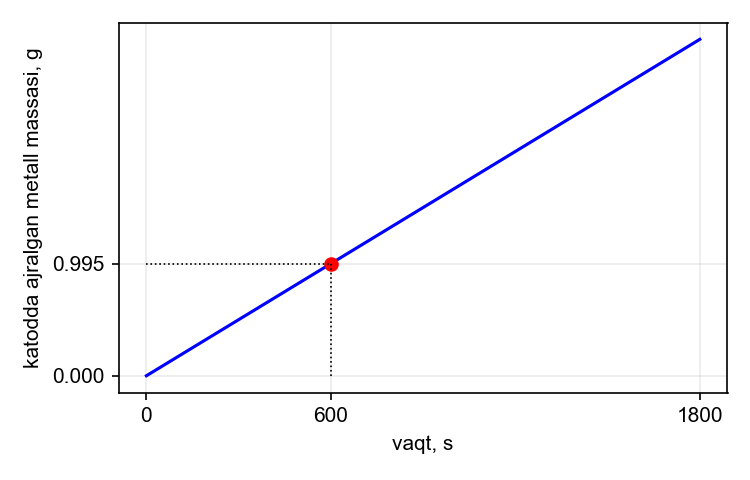
\includegraphics[width=0.86\linewidth]{rasmlar/gen/fa_v16_0.png}\end{center}
Xuddi shu sharoitda 1800 s da ajralgan metall \textbf{massasini (g) toping.}

\noindent A)~\textsl{5,969} \hfill B)~\textsl{1,492} \hfill C)~\textsl{2,984} \hfill D)~\textsl{1,99}\par
\vspace{4pt}
\noindent\textbf{14.} Rasmdagi o`zgarishlar zanjirida \textit{X} moddaning \textbf{formulasini aniqlang.}
\begin{center}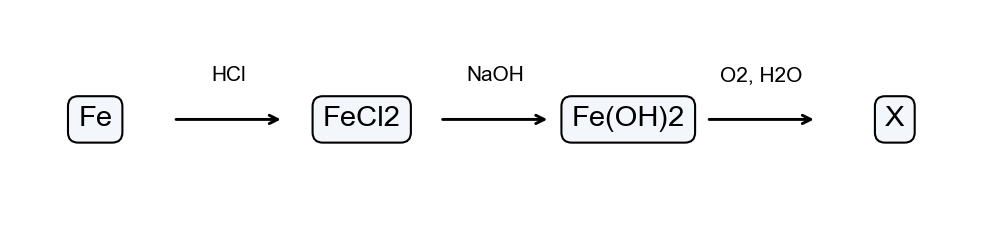
\includegraphics[width=0.86\linewidth]{rasmlar/gen/ci_509279.png}\end{center}

\noindent A)~\textsl{Fe(OH)\textsubscript{3}} \hfill B)~\textsl{FeCl\textsubscript{2}} \hfill C)~\textsl{SO\textsubscript{3}} \hfill D)~\textsl{Fe(OH)\textsubscript{2}}\par
\vspace{4pt}
\noindent\textbf{15.} Cu $\to$ ? $\to$ ? $\to$ ? o`zgarishlar zanjirida (reagentlar: O\textsubscript{2}, H\textsubscript{2}SO\textsubscript{4}, NaOH) 1-bosqichda hosil bo`ladigan modda \textbf{formulasini toping.}

\noindent A)~\textsl{Na\textsubscript{2}SO\textsubscript{3}} \hfill B)~\textsl{Ca(OH)\textsubscript{2}} \hfill C)~\textsl{NaCl} \hfill D)~\textsl{CuO}\par
\vspace{4pt}
\noindent\textbf{16.} NH\textsubscript{3} + H\textsubscript{3}PO\textsubscript{4} $\to$ NH\textsubscript{4}H\textsubscript{2}PO\textsubscript{4} jarayoni uchun 4,48 l (n.sh.) NH\textsubscript{3} olingan (unum 90\%). NH\textsubscript{4}H\textsubscript{2}PO\textsubscript{4} \textbf{miqdorini (mol) aniqlang.}

\noindent A)~\textsl{0,2} \hfill B)~\textsl{0,36} \hfill C)~\textsl{0,09} \hfill D)~\textsl{0,18}\par
\vspace{4pt}
\noindent\textbf{17.} Cu(NO\textsubscript{3})\textsubscript{2} qizdirilganda qanday moddalar hosil bo`ladi?

\noindent\begin{tabular}{@{}p{0.47\linewidth}@{}p{0.47\linewidth}@{}}
A)~\textsl{Ag, NO\textsubscript{2} va O\textsubscript{2}} & B)~\textsl{ZnO, NO\textsubscript{2} va O\textsubscript{2}} \\
C)~\textsl{CuO, NO\textsubscript{2} va O\textsubscript{2}} & D)~\textsl{N\textsubscript{2}O va H\textsubscript{2}O} \\
\end{tabular}\par
\vspace{4pt}
\noindent\textbf{18.} 4FeS\textsubscript{2} + 11O\textsubscript{2} $\to$ 2Fe\textsubscript{2}O\textsubscript{3} + 8SO\textsubscript{2} reaksiyasida 12 g FeS\textsubscript{2} ishtirok etdi. SO\textsubscript{2} \textbf{hajmini (l, n.sh.) toping.}

\noindent A)~\textsl{1,12} \hfill B)~\textsl{4,48} \hfill C)~\textsl{8,96} \hfill D)~\textsl{2,24}\par
\vspace{4pt}
\noindent\textbf{19.} 17 g AgNO\textsubscript{3} to`liq parchalanguncha qizdirildi. Qattiq qoldiq \textbf{massasini (g) aniqlang.}

\noindent A)~\textsl{10,8} \hfill B)~\textsl{17} \hfill C)~\textsl{21,6} \hfill D)~\textsl{5,4}\par
\vspace{4pt}
\noindent\textbf{20.} C\textsubscript{3}H\textsubscript{8} + 5O\textsubscript{2} $\to$ 3CO\textsubscript{2} + 4H\textsubscript{2}O jarayoni uchun 8,96 l (n.sh.) C\textsubscript{3}H\textsubscript{8} olingan. CO\textsubscript{2} \textbf{hajmini (l, n.sh.) aniqlang.}

\noindent A)~\textsl{26,88} \hfill B)~\textsl{2,99} \hfill C)~\textsl{53,76} \hfill D)~\textsl{13,44}\par
\vspace{4pt}
\noindent\textbf{21.} CH\textsubscript{3}--CH(CH\textsubscript{3})--CH(C\textsubscript{2}H\textsubscript{5})--CH\textsubscript{2}--CH\textsubscript{3} birikmaning sistematik nomi qaysi qatorda to`g`ri keltirilgan?

\noindent\begin{tabular}{@{}p{0.47\linewidth}@{}p{0.47\linewidth}@{}}
A)~\textsl{2-metil-3-etilpentan} & B)~\textsl{3-etil-2-metilpentan} \\
C)~\textsl{3-izopropilpentan} & D)~\textsl{2,3-dietilbutan} \\
\end{tabular}\par
\vspace{4pt}
\noindent\textbf{22.} 9,2 g toluoldan benzoy kislota olishda unum 75\% bo`lsa, mahsulot \textbf{massasini (g) aniqlang} (boshlang`ich modda massasi 9,2 g).

\noindent A)~\textsl{12,2} \hfill B)~\textsl{18,3} \hfill C)~\textsl{9,15} \hfill D)~\textsl{6,9}\par
\vspace{4pt}
\noindent\textbf{23.} C\textsubscript{2}H\textsubscript{4} + H\textsubscript{2}O (H\textsuperscript{+}) reaksiyasi natijasida qaysi organik modda hosil bo`ladi?

\noindent\begin{tabular}{@{}p{0.47\linewidth}@{}p{0.47\linewidth}@{}}
A)~\textsl{metan} & B)~\textsl{etanol} \\
C)~\textsl{etilatsetat} & D)~\textsl{benzoy kislota} \\
\end{tabular}\par
\vspace{4pt}
\noindent\textbf{24.} 44 g CH\textsubscript{3}CHO dan quyidagi ikki bosqichda C\textsubscript{2}H\textsubscript{4} olinadi: 1) CH\textsubscript{3}CHO + H\textsubscript{2} $\to$ C\textsubscript{2}H\textsubscript{5}OH (unum 75\%); 2) C\textsubscript{2}H\textsubscript{5}OH $\to$ C\textsubscript{2}H\textsubscript{4} + H\textsubscript{2}O (unum 75\%). Oxirgi mahsulot C\textsubscript{2}H\textsubscript{4} ning \textbf{hajmini (l, n.sh.) toping.}

\noindent A)~\textsl{12,6} \hfill B)~\textsl{16,8} \hfill C)~\textsl{22,4} \hfill D)~\textsl{25,2}\par
\vspace{4pt}
\noindent\textbf{25.} C\textsubscript{4}H\textsubscript{10}O oddiy efirlarning izomerlari soni nechta?

\noindent A)~\textsl{4} \hfill B)~\textsl{3} \hfill C)~\textsl{2} \hfill D)~\textsl{5}\par
\vspace{4pt}
\noindent\textbf{26.} 17,6 g CH\textsubscript{3}COOC\textsubscript{2}H\textsubscript{5} dan quyidagi ikki bosqichda Na\textsubscript{2}CO\textsubscript{3} olinadi: 1) CH\textsubscript{3}COOC\textsubscript{2}H\textsubscript{5} + NaOH $\to$ CH\textsubscript{3}COONa + C\textsubscript{2}H\textsubscript{5}OH (unum 75\%); 2) CH\textsubscript{3}COONa + NaOH $\to$ CH\textsubscript{4} + Na\textsubscript{2}CO\textsubscript{3} (unum 90\%). Oxirgi mahsulot Na\textsubscript{2}CO\textsubscript{3} ning \textbf{massasini (g) toping.}

\noindent A)~\textsl{19,08} \hfill B)~\textsl{15,9} \hfill C)~\textsl{21,2} \hfill D)~\textsl{14,31}\par
\vspace{4pt}
\noindent\textbf{27.} Uglevodlar haqida qaysi fikrlar to`g`ri? 1) Glyukoza "kumush ko`zgu" reaksiyasini beradi; 2) Selluloza $\beta$-glyukoza qoldiqlaridan iborat; 3) Fruktoza ketospirt; 4) Glyukoza gidrolizlanadi

\noindent A)~\textsl{1, 2, 3} \hfill B)~\textsl{2, 3, 4} \hfill C)~\textsl{3, 4} \hfill D)~\textsl{2, 3}\par
\vspace{4pt}
\noindent\textbf{28.} Aminlar, aminokislotalar va oqsillar haqida qaysi fikrlar to`g`ri? 1) Oqsillar biuret reaksiyasini beradi; 2) Nitrobenzoldan anilin Zinin reaksiyasi bilan olinadi; 3) Dipeptidda 2 ta peptid bog` bor; 4) Aminlar kuchsiz asoslar xossasini namoyon qiladi

\noindent A)~\textsl{3, 4} \hfill B)~\textsl{2, 3} \hfill C)~\textsl{1, 3, 4} \hfill D)~\textsl{1, 2, 4}\par
\vspace{4pt}
\noindent\textbf{29.} Yuqori molekulyar birikmalar haqida qaysi fikrlar to`g`ri? 1) Kapron poliamid tola; 2) Polimerning M = zveno M $\cdot$ polimerlanish darajasi; 3) Teflon --- polivinilxlorid; 4) Fenolformaldegid smola polikondensatsiya mahsuloti

\noindent A)~\textsl{1, 2, 4} \hfill B)~\textsl{1, 2, 3} \hfill C)~\textsl{2, 4} \hfill D)~\textsl{1, 4}\par
\vspace{4pt}
\noindent\textbf{30.} 100 g 30\% li va 100 g 40\% li NaOH eritmalari aralashtirildi. Yangi eritmaning massa \textbf{ulushini (\%) toping.}

\noindent A)~\textsl{70} \hfill B)~\textsl{35} \hfill C)~\textsl{31,5} \hfill D)~\textsl{38,5}\par
\vspace{4pt}
\noindent\textbf{31.} Kimyo laboratoriyasida ishlash qoidalari haqida qaysi fikrlar to`g`ri? 1) Ishqor teriga tushsa, qo`l suv bilan yuviladi; 2) Probirka qizdirilganda og`zi odamga qaratilmaydi; 3) Zaharli gaz ajraladigan tajriba mo`rili shkafda o`tkaziladi; 4) Konsentrlangan kislotani suvga ohista, aralashtirib quyiladi

\noindent\begin{tabular}{@{}p{0.47\linewidth}@{}p{0.47\linewidth}@{}}
A)~\textsl{2, 3, 4} & B)~\textsl{1, 3, 4} \\
C)~\textsl{1, 2, 3, 4} & D)~\textsl{1, 2, 4} \\
\end{tabular}\par
\vspace{4pt}
\noindent\textbf{32.} Rasmdagi asbob bilan qaysi aralashmani ajratish mumkin?
\begin{center}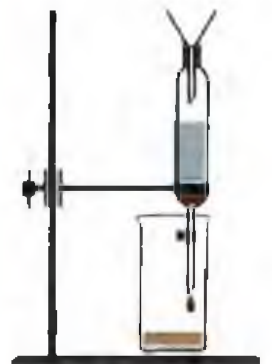
\includegraphics[width=0.86\linewidth]{rasmlar/darslik/d_ajratgich.png}\end{center}

\noindent\begin{tabular}{@{}p{0.47\linewidth}@{}p{0.47\linewidth}@{}}
A)~\textsl{suv va qum} & B)~\textsl{suv va etanol} \\
C)~\textsl{osh tuzi eritmasi} & D)~\textsl{suv va kerosin   ---} \\
\end{tabular}\par
\vspace{4pt}
\end{multicols}
\medskip
\noindent\setlength{\fboxsep}{0pt}\fbox{\begin{tabular}{p{0.74\linewidth}|p{0.2\linewidth}}
\parbox[t]{0.72\linewidth}{\vspace{3pt}\textbf{Topshiriqlar (33--35) va javob variant (A--F)larini o`zaro to`g`ri moslashtiring.} K\textsubscript{2}CO\textsubscript{3} va MgCO\textsubscript{3} dan iborat 39 g aralashma mo`l xlorid kislota bilan to`liq reaksiyaga kirishdi.
\vspace{3pt}} & \parbox[t]{0.19\linewidth}{\vspace{3pt}A~\textsl{292}\\[3pt]
B~\textsl{8,96}\\[3pt]
C~\textsl{35,95}\\[3pt]
D~\textsl{28,76}\\[3pt]
E~\textsl{17,92}\\[3pt]
F~\textsl{584}}\\ \hline
\parbox[t]{0.72\linewidth}{\vspace{2pt}\textbf{33. Ajralgan gaz hajmini (l, n.sh.) aniqlang.}\vspace{2pt}} & \\ \hline
\parbox[t]{0.72\linewidth}{\vspace{2pt}\textbf{34. Aralashmani to`liq eritish uchun sarflangan 10\% li HCl eritmasining massasini (g) aniqlang (M(HCl) = 36,5 g/mol).}\vspace{2pt}} & \\ \hline
\parbox[t]{0.72\linewidth}{\vspace{2pt}\textbf{35. Reaksiyadan so`ng eritmadagi tuzlar umumiy massasini (g) aniqlang.}\vspace{2pt}} & 
\end{tabular}}
\par\bigskip
\noindent\textbf{36.} KMnO\textsubscript{4} + K\textsubscript{2}SO\textsubscript{3} + H\textsubscript{2}O $\to$ MnO\textsubscript{2} + K\textsubscript{2}SO\textsubscript{4} + KOH reaksiya tenglamasini tenglang va barcha koeffitsiyentlar \textbf{yig`indisini aniqlang.}
\javob
\noindent\textbf{37.} 8,5 g H\textsubscript{2}O\textsubscript{2} reaksiyaga kirishdi (2H\textsubscript{2}O\textsubscript{2} $\to$ 2H\textsubscript{2}O + O\textsubscript{2}). Ajralgan O\textsubscript{2} \textbf{hajmini (l, n.sh.) hisoblang} (unum 80\%).
\javob
\noindent\textbf{38.} 100 m\textsuperscript{3} suvda Ca(HCO\textsubscript{3})\textsubscript{2} konsentratsiyasi 20 mol/m\textsuperscript{3}, Mg(HCO\textsubscript{3})\textsubscript{2} niki 20 mol/m\textsuperscript{3}. Suvni Ca(OH)\textsubscript{2} bilan to`liq yumshatish uchun Ca(OH)\textsubscript{2} ning \textbf{massasini (kg) hisoblang.}
\javob
\noindent\textbf{39.} 9,2 g etanol avval sirka aldegidgacha (unum 80\%), so`ng sirka kislotagacha (unum 60\%) oksidlandi; hosil bo`lgan kislota mo`l etanol bilan efirlandi (unum 100\%). Etilatsetat \textbf{massasini (g) toping.}
\javob
\noindent\textbf{40.} 14,8 g propion kislota va 9,2 g etanol dan 60\% unum bilan murakkab efir olindi. Efir \textbf{massasini (g) toping.}
\javob
\par\bigskip\begin{center}\textbf{\fontsize{13}{15}\selectfont YOZMA ISH}\end{center}
\noindent\textbf{41.} \textbf{Topshiriqni bajarish jarayonida barcha reaksiya tenglamalarini yozing. Miqdoriy va arifmetik hisoblashlarni (unga asos bo`lgan usul yoki formulani ko`rsatgan holda) uzviy ketma-ketlikda bajaring.}\par\smallskip
Tabiiy mis ikki izotopdan iborat: \textsuperscript{63}Cu (70\%) va \textsuperscript{65}Cu (30\%). 6,4 g shu element namunasi olingan (\textit{Z} = 29, N\textsubscript{A} = 6,02$\cdot$10\textsuperscript{23}).\par
\noindent 1)Elementning o`rtacha nisbiy atom massasini hisoblang.\par
\noindent 2)Namunadagi atomlarning umumiy miqdorini (mol) toping. Namunadagi protonlar sonini (mol) ham toping.\par
\noindent 3)Og`irroq izotop (\textsuperscript{65}Cu) atomlarining miqdorini (mol) hisoblang.\par
\noindent 4)Namunadagi neytronlarning umumiy miqdorini (mol) toping. Bitta atom massasini (g) ham hisoblang.\par
\noindent 5)Namunadagi atomlar sonini (10\textsuperscript{23} birligida) aniqlang. Namunadagi protonlar sonining neytronlar soniga nisbatini ham toping.\par
\diqqat{Mazkur topshiriq kengaytirilgan javobni talab etib, uning yechilish usuli va shu usul asosidagi barcha hisoblash amallari javoblar varaqasida aks etishi lozim.}
\noindent\textbf{42.} Quyidagi o`zgarishlar zanjirida \textit{X}, \textit{Y}, \textit{Z} noma'lum organik moddalar:\par
\[\setlength{\fboxsep}{0pt}\text{C\textsubscript{2}H\textsubscript{4}Br\textsubscript{2}}\xrightarrow{\text{KOH (spirtli)}}\text{\textit{X}}\xrightarrow{\text{C (aktiv), 600 \textdegree{}C}}\text{\textit{Y}}\xrightarrow{\text{CH\textsubscript{3}Cl, AlCl\textsubscript{3}}}\text{C\textsubscript{6}H\textsubscript{5}CH\textsubscript{3}}\]
\noindent 1)C\textsubscript{2}H\textsubscript{4}Br\textsubscript{2} $\to$ \textit{X} : reaksiya tenglamasini yozing; hosil bo`lgan moddani nomlang.\par
\noindent 2)\textit{X} $\to$ \textit{Y} : reaksiya tenglamasini yozing; hosil bo`lgan moddani nomlang.\par
\noindent 3)\textit{Y} $\to$ C\textsubscript{6}H\textsubscript{5}CH\textsubscript{3} : reaksiya tenglamasini yozing; hosil bo`lgan moddani nomlang.\par
\diqqat{Mazkur topshiriq kengaytirilgan javobni talab etib, uning yechilish usuli va shu usul asosidagi barcha hisoblash amallari javoblar varaqasida aks etishi lozim.}
\noindent\textbf{43.} \textbf{Topshiriqni bajarish jarayonida barcha reaksiya tenglamalarini yozing. Miqdoriy va arifmetik hisoblashlarni (unga asos bo`lgan usul yoki formulani ko`rsatgan holda) uzviy ketma-ketlikda bajaring.}\par\smallskip
6,2 g qizil fosfor mo`l kislorodda yondirildi, hosil bo`lgan oksid suvda to`liq eritildi (ortofosfat kislota). Eritmaga 0,4 mol NaOH qo`shildi.\par
\noindent 1)Reaksiya tenglamalarini yozing. Hosil bo`lgan P\textsubscript{2}O\textsubscript{5} massasini (g) hisoblang.\par
\noindent 2)Hosil bo`lgan H\textsubscript{3}PO\textsubscript{4} massasini (g) toping. Kislotada fosforning massa ulushini (\%) ham hisoblang.\par
\noindent 3)Eritmada qanday tuz hosil bo`lganini aniqlang va uning massasini (g) hisoblang.\par
\noindent 4)Hosil bo`lgan eritmani to`liq neytrallash uchun yana qancha NaOH (g) kerak (Na\textsubscript{2}HPO\textsubscript{4} $\to$ Na\textsubscript{3}PO\textsubscript{4})?\par
\noindent 5)Hosil bo`lgan tuzning 10\% li eritmasi massasini (g) hisoblang.\par
\diqqat{Mazkur topshiriq kengaytirilgan javobni talab etib, uning yechilish usuli va shu usul asosidagi barcha hisoblash amallari javoblar varaqasida aks etishi lozim.}
\newpage
\noindent\textbf{\fontsize{13}{15}\selectfont Nazorat testi}\ \textit{$\cdot$ 16-variant}\hfill \textbf{Javoblar kaliti}\par\smallskip\hrule\smallskip
\textit{Faqat o`qituvchi uchun.}\par\medskip
\noindent\textbf{1--32-savollar}\par\smallskip
\noindent\begin{tabular}{|c|c|c|c|c|c|c|c|c|c|c|c|c|c|c|c|}\hline
\textbf{1} & \textbf{2} & \textbf{3} & \textbf{4} & \textbf{5} & \textbf{6} & \textbf{7} & \textbf{8} & \textbf{9} & \textbf{10} & \textbf{11} & \textbf{12} & \textbf{13} & \textbf{14} & \textbf{15} & \textbf{16}\\\hline
\textsl{B} & \textsl{C} & \textsl{D} & \textsl{A} & \textsl{C} & \textsl{D} & \textsl{C} & \textsl{B} & \textsl{D} & \textsl{B} & \textsl{A} & \textsl{C} & \textsl{C} & \textsl{A} & \textsl{D} & \textsl{D}\\\hline
\textbf{17} & \textbf{18} & \textbf{19} & \textbf{20} & \textbf{21} & \textbf{22} & \textbf{23} & \textbf{24} & \textbf{25} & \textbf{26} & \textbf{27} & \textbf{28} & \textbf{29} & \textbf{30} & \textbf{31} & \textbf{32}\\\hline
\textsl{C} & \textsl{B} & \textsl{A} & \textsl{A} & \textsl{B} & \textsl{C} & \textsl{B} & \textsl{A} & \textsl{B} & \textsl{D} & \textsl{A} & \textsl{D} & \textsl{A} & \textsl{B} & \textsl{C} & \textsl{D}\\\hline
\end{tabular}\par\medskip
\noindent\textbf{33--35-savollar}\par\smallskip
\noindent\begin{tabular}{|c|c|c|}\hline \textbf{No} & \textbf{Javob} & \textbf{Qiymat}\\\hline
33 & \textsl{B} & 8,96\\\hline
34 & \textsl{A} & 292\\\hline
35 & \textsl{C} & 35,95\\\hline
\end{tabular}\par\medskip
\noindent\textbf{36--40-savollar}\par\smallskip
\noindent\begin{tabular}{|c|c|}\hline \textbf{No} & \textbf{To`g`ri javob}\\\hline
36 & 13\\\hline
37 & 2,24\\\hline
38 & 444\\\hline
39 & 8,45\\\hline
40 & 12,24\\\hline
\end{tabular}\par\medskip
\noindent\textbf{41--43-topshiriqlar: qisqa yechim}\par\smallskip
\noindent\textbf{41-topshiriq.}\par
\noindent 1) Ar = (63$\cdot$70 + 65$\cdot$30)/100 = \textbf{63,6}\par
\noindent 2) n = 6,4/63,6 = \textbf{0,101 mol}; n(p) = \textit{Z}$\cdot$n = 29$\cdot$0,101 = \textbf{2,918 mol}\par
\noindent 3) n(\textsuperscript{65}Cu) = 0,101$\cdot$30/100 = \textbf{0,03 mol}\par
\noindent 4) N(neytron) = $\Sigma$ (A $-$ \textit{Z})$\cdot$ulush: \textbf{3,482 mol}; m(atom) = 63,6/(6,02$\cdot$10\textsuperscript{23}) = \textbf{10,56$\cdot$10\textsuperscript{$-$23} g}\par
\noindent 5) N = n$\cdot$N\textsubscript{A} = 0,101$\cdot$6,02$\cdot$10\textsuperscript{23} = \textbf{0,61$\cdot$10\textsuperscript{23}}; n(p)/n(n) = 2,918/3,482 = \textbf{0,838}\par
\noindent Jami: M 15 + A 10 = 25 ball.\par
\noindent\textbf{42-topshiriq.}\par
\noindent 1) C\textsubscript{2}H\textsubscript{4}Br\textsubscript{2} + KOH (spirtli) $\to$ C\textsubscript{2}H\textsubscript{2} (asetilen)\par
\noindent 2) C\textsubscript{2}H\textsubscript{2} + C (aktiv), 600 \textdegree{}C $\to$ C\textsubscript{6}H\textsubscript{6} (benzol)\par
\noindent 3) C\textsubscript{6}H\textsubscript{6} + CH\textsubscript{3}Cl, AlCl\textsubscript{3} $\to$ C\textsubscript{6}H\textsubscript{5}CH\textsubscript{3} (toluol)\par
\noindent Jami 25 ball.\par
\noindent\textbf{43-topshiriq.}\par
\noindent 1) 4P + 5O\textsubscript{2} $\to$ 2P\textsubscript{2}O\textsubscript{5}: n(P\textsubscript{2}O\textsubscript{5}) = 0,1 mol $\to$ \textbf{14,2 g}\par
\noindent 2) P\textsubscript{2}O\textsubscript{5} + 3H\textsubscript{2}O $\to$ 2H\textsubscript{3}PO\textsubscript{4}: n = 0,2 mol $\to$ \textbf{19,6 g}; $\omega$(P) = 31/98 = \textbf{31,6\%}\par
\noindent 3) H\textsubscript{3}PO\textsubscript{4} : NaOH = 1 : 2 $\to$ \textbf{Na\textsubscript{2}HPO\textsubscript{4}} 0,2 mol = \textbf{28,4 g}\par
\noindent 4) Na\textsubscript{2}HPO\textsubscript{4} + NaOH $\to$ Na\textsubscript{3}PO\textsubscript{4} + H\textsubscript{2}O: 0,2 mol $\cdot$ 40 = \textbf{8 g}\par
\noindent 5) m(eritma) = 28,4/0,1 = \textbf{284 g}\par
\noindent Jami: M 15 + A 10 = 25 ball.\par
\par\bigskip\noindent\textbf{Mavzular taqsimoti}\par\smallskip
{\small\noindent\begin{longtable}{|c|p{7.2cm}|p{5.4cm}|c|}\hline \textbf{No} & \textbf{Mavzu} & \textbf{Tekshiriladigan ko`nikma} & \textbf{Ball}\\\hline
1 & 11-sinf (Mendeleyev--Klapeyron) & Hisoblash va masala yechish & 1\\\hline
2 & 11-sinf (Mendeleyev--Klapeyron) & Hisoblash va masala yechish & 1\\\hline
3 & 8-sinf; Tirkashev II bob (kimyoviy bog`lanish) & Bilim va tushunish & 1\\\hline
4 & 8-sinf; Tirkashev VI bob & Jadval tahlili & 1\\\hline
5 & 8-sinf; Tirkashev \textit{V} bob (oksidlanish darajasi) & Bilim va tushunish & 1\\\hline
6 & 8-sinf (ortiqcha modda masalasi) & Hisoblash va masala yechish & 1\\\hline
7 & 8-sinf; Tirkashev VI bob & Jadval tahlili & 1\\\hline
8 & 11-sinf 4-bob (normal konsentratsiya) & Hisoblash va masala yechish & 1\\\hline
9 & Tirkashev \textit{V} bob (OQR, jadval) & Jadval tahlili & 1\\\hline
10 & Tirkashev VI bob & Hisoblash va masala yechish & 1\\\hline
11 & 9-sinf (gidroliz); Tirkashev IV bob & Bilim va tushunish & 1\\\hline
12 & Tirkashev III bob (kristallogidrat) & Hisoblash va masala yechish & 1\\\hline
13 & 11-sinf (Faradey qonuni, grafik) & Grafik tahlili & 1\\\hline
14 & 9-sinf (genetik bog`lanish) & Rasm bo`yicha tahlil & 1\\\hline
15 & 8-sinf; 9-sinf (genetik bog`lanish) & Bilim va tushunish & 1\\\hline
16 & 9-sinf; Tirkashev (mineral o`g`itlar/nodir gazlar, hisob) & Hisoblash va masala yechish & 1\\\hline
17 & Tashev (nitratlar) & Bilim va tushunish & 1\\\hline
18 & 9-sinf; Tirkashev (S/SO\textsubscript{2}/H\textsubscript{2}SO\textsubscript{4}, hisob) & Hisoblash va masala yechish & 1\\\hline
19 & Tashev (nitratlar termik parchalanishi) & Hisoblash va masala yechish & 1\\\hline
20 & 10-sinf (alkan, hisob) & Hisoblash va masala yechish & 1\\\hline
21 & 10-sinf (nomenklatura \S{}6, \S{}11, \S{}20, \S{}24--26) & Bilim va tushunish & 1\\\hline
22 & 10-sinf \S{}16, \S{}23, \S{}33 & Hisoblash va masala yechish & 1\\\hline
23 & 10-sinf (olinish usullari) & Bilim va tushunish & 1\\\hline
24 & 10-sinf (ikki bosqichli hisob) & Hisoblash va masala yechish & 1\\\hline
25 & 10-sinf \S{}6, \S{}12, \S{}20, \S{}28 (izomeriya) & Bilim va tushunish & 1\\\hline
26 & 10-sinf (ikki bosqichli hisob) & Hisoblash va masala yechish & 1\\\hline
27 & 10-sinf (mavzuga oid paragraflar); Abdusamatov & Bilim va tushunish & 1\\\hline
28 & 10-sinf (mavzuga oid paragraflar); Abdusamatov & Bilim va tushunish & 1\\\hline
29 & 10-sinf (mavzuga oid paragraflar); Abdusamatov & Bilim va tushunish & 1\\\hline
30 & Tirkashev III bob (eritmalar) & Hisoblash va masala yechish & 1\\\hline
31 & 7-sinf (xavfsizlik qoidalari); 10-sinf lab. & Bilim va tushunish & 1\\\hline
32 & 7-sinf (10-rasm) & Rasm bo`yicha tahlil & 1\\\hline
33--35 & Aralash masala (moslashtirish) & Ko`p bosqichli hisob & 3\\\hline
36--40 & Qisqa javobli masalalar & Hisoblash & 5\\\hline
41--43 & Yozma ish & Usul va hisob (M, A) & 75\\\hline
\end{longtable}}
\end{document}
